\documentclass{article}
\usepackage{graphicx} % Required for inserting images
\usepackage[colorlinks=true, allcolors=blue]{hyperref}
\usepackage{titlesec}
\usepackage[square,numbers]{natbib}
\usepackage{geometry}
\geometry{
a4paper,
total={170mm,257mm},
left=20mm,
top=20mm,
}
\graphicspath{ {./images/} }

\bibliographystyle{dinat}

\title{Unit 23}
\author{Chris Hadden}
\date{}

\begin{document}

\maketitle
\section{D1 Evaluate the potential repurposing of your solution to other business sectors}
In this report we will outline how our Patient Diagnosis chatbot that we defined in Task 4 P3 could be used in other technological areas so that we can get the most value from our own technology. This is what is known as repurposing, taking an existing technology and adapting it for another related purpose.
\smallbreak
\section{Assessing prior art}
Here we are going to report on our research to find other implementations of diagnosis chatbots to see if other development teams have discovered repurposed implementations and if we can do the same with ours.
\smallbreak
A general point about GP chat points has been made by Noel Kennedy in that "A chatbot designed for the Healthcare industry to answer calls from the general public to
their GP greatly improves the efficiency of obtaining appointments, getting sound medical advice and reduces the workload on the staff in the GP’s surgery. Would this same technology be of use in the retail or finance sector to reduce call waiting times?" \cite{Noel}

This is a fair point and may point us in a lucrative area of research.
\smallbreak

\subsection{Comparing Physician and Artificial Intelligence Chatbot Responses to Patient Questions Posted to a Public Social Media Forum}
In the research paper Comparing Physician and Artificial Intelligence Chatbot Responses to Patient Questions Posted to a Public Social Media Forum\cite{bedside} one of the conclusions they came up with was that "a chatbot generated quality and empathetic responses to patient questions posed in an online forum" and "Further exploration of this technology is warranted in clinical settings, such as using chatbot to draft responses that physicians could then edit". In essence they are saying that the chatbot had a great bedside manner. This could lead us to thinking about using the chatbot as a therapist of some kind.


\subsection{Bookings}
One of the main uses of our chatbot was not just diagnosis but also possibly to make a booking to see GP. Looking in to chatbots that can make bookings we have found a plethora of businesses that have already been setup to do just this.\cite{futr}\cite{booking}\cite{velma} The example from booking.com is interesting as well as they mention "In September 2017, Finnair launched its first chatbot via Facebook Messenger. Nicknamed Finn, it can sell flights, calculate how much baggage a passenger can take and respond to questions." All of this is very advanced and shows that our chatbot could take on quite a lot.

\subsection{Expanding on diagnosis}
The main use of our chatbot was to help with diagnosis of the patient's issues with a view to making the GP's work quicker and easier. This is a perfect use of a chatbot in that it augments the GPs work and allows them to assess more patients, especially as the chatbot's work can be done while waiting for the GP. 
This diagnosis facility could be used in other areas where a client knows what the symptoms of a problem are and need help to diagnose what the actual problem is. This is sometimes called Root Cause Analysis, and there are a number of chatbots that can already do this. \cite{gyan}\cite{devops}

\section{Assessing our chatbot}
At this point we want to list out the main features in our chatbot, and list them in a fairly subjective ranking. Doing this will mean that we can assert what the chatbot's strengths and weaknesses are and see if we can tie them up with any of the prior art to come up with any new creative applications for the chatbot.
\smallbreak
This is not an exhaustive list, but from best to worst we have:
\begin{enumerate}
    \item Bot can diagnose patient problems
    \item Bot saves time for GP
    \item Bot can take action on behalf of patient like making a booking
    \item Bot can be empathetic
    \item Bot may be seen as soulless
    \item Bot may make incorrect diagnosis and as such needs to be monitored
    \item Bot may remove certain jobs, and those employees may not be able to or unwilling to retrain
\end{enumerate}

\subsection{Bot can diagnose patient problems / Bot saves time for GP}

This is very much the highlight of our chat bot. The act of diagnosis is an act that can be replicated and reused in other domains. 
The usual flow when diagnosing issues would be a bit like this.
\begin{center} 
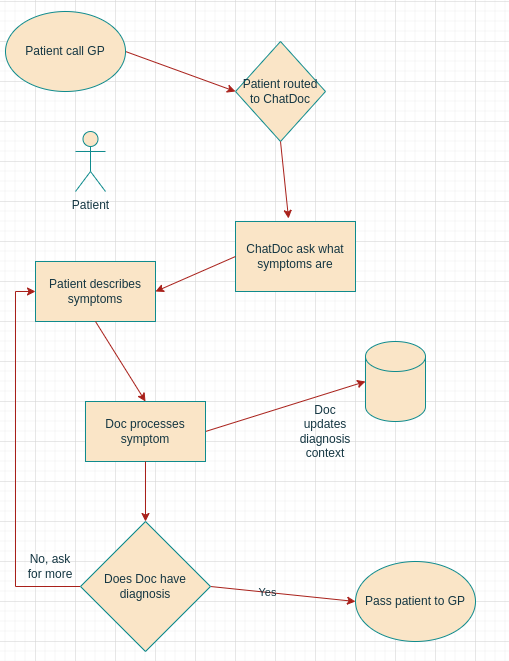
\includegraphics[scale=0.5]{PatientFlow}
\end{center}
This is an iterative approach where the chatbot asks more questions until it can make a reliable diagnosis. This same process could be used in many other scenarios such as trying to diagnose a defective engine or to assess drainage problems on a farm. As long as the chatbot has the correct training then there is no limit to where this process could be applied. This ties in very well with what we saw in the prior art where chatbots are used in Root Cause Analysis\cite{gyan}\cite{devops}

\subsection{Bot can take action on behalf of patient like making a booking}
This action is very much like a basic receptionist job. It is easy to automate repetitive and well defined action such as setting up a meeting or requesting a repeat prescription, and this can also shorten waiting times for customers as they are dealt with quickly and will never be in the queue infront of other customers. This ties in very well with the booking prior art we saw previously. Arguably as this is so simple and it seems like there are many other companies already doing this, that it is already a crowded market and if we were to repurpose our chatbot to automate these admin tasks then we would need to find something more advanced or more niche to be of any use.

\subsection{Bot can be empathetic / Bot may be seen as soulless}
This was a concern that we had when we made the case for our chatbot, but as we have seen it turns out that chatbots by their very nature come across as very empathetic \cite{bedside}. Having a chatbot that not only understands patients medical needs but seems empathetic and by it's very nature has infinite patience lends itself to areas such a therapy and psychology. There is a danger in using a chatbot this way in that it could create a very personal relationship with a patient and if not monitored then it could lead to unexpected and worrying places. However with the correct monitoring in place, it could be a very powerful tool, especially as it it extremely hard for people to get help with mental health issues on the NSH due to a lack of professionals. 

\subsection{Bot may make incorrect diagnosis and as such needs to be monitored / Bot may remove certain jobs, and those employees may not be able to or unwilling to retrain}
These were two weaknesses that sort of self correct each other. They are not strictly to do with repurposing the technology but more to do with repurposing people. As we have seen previously and in the section on therapy bots, these bots still need to be monitored. As certain jobs are being done away with due to technology, new opportunities arise from the technology and with some retraining, it would be quite easy to fill those jobs with the ones that have been lost.

\bibliography{bibliography}
\end{document}
s